\documentclass[11pt,addpoints,answers]{exam}

%-----------------------------------------------------------------------------
% PACKAGES AND OTHER DOCUMENT CONFIGURATIONS
%-----------------------------------------------------------------------------

\usepackage[margin=1in]{geometry}
\usepackage{amsmath, amsfonts}
\usepackage{enumerate}
\usepackage{graphicx}
\usepackage{titling}
\usepackage{url}
\usepackage{xfrac}
\usepackage{natbib}
\usepackage{amssymb}
\usepackage{amsthm}
\usepackage{paralist}
\usepackage{epstopdf}
\usepackage{tabularx}
\usepackage{longtable}
\usepackage{multirow}
\usepackage{multicol}
\usepackage[colorlinks=true,urlcolor=blue]{hyperref}
\usepackage{algorithm}
\usepackage{algorithmicx}
\usepackage[noend]{algpseudocode}
\usepackage{float}
\usepackage{enumerate}
\usepackage{array}
\usepackage{environ}
\usepackage{times}
\usepackage{textcomp}
\usepackage{caption}
\usepackage{parskip} % For NIPS style paragraphs.
\usepackage[compact]{titlesec} % Less whitespace around titles
\usepackage[inline]{enumitem} % For inline enumerate* and itemize*
\usepackage{datetime}
\usepackage{comment}
% \usepackage{minted}
\usepackage{lastpage}
\usepackage{color}
\usepackage{xcolor}
\usepackage[final]{listings}
\usepackage{tikz}
\usetikzlibrary{shapes,decorations}
\usepackage{framed}
\usepackage{booktabs}
\usepackage{cprotect}
\usepackage{verbatim}
\usepackage{verbatimbox}
\usepackage{multicol}
\usepackage{hyperref}
\usepackage{subcaption}
\usepackage{mathtools} % For drcases
\usepackage{cancel}
\usepackage[many]{tcolorbox}
\usepackage{soul}
\usepackage[bottom]{footmisc}
\usepackage{bm}
\usepackage{wasysym}
\usepackage[utf8]{inputenc}
\usepackage{tikz}
\usetikzlibrary{arrows}
\usetikzlibrary{arrows.meta}
\usetikzlibrary{shapes.geometric}
\usetikzlibrary{positioning, arrows, automata, calc}
\usepackage{transparent}

\newtcolorbox[]{your_solution}[1][]{
    % breakable,
    enhanced,
    nobeforeafter,
    colback=white,
    title=Your Answer,
    sidebyside align=top,
    box align=top,
    #1
}

%%%%%%%%%%%%%%%%%%%%%%%%%%%%%%%%%%%%%%%%%%%
% Formatting for \CorrectChoice of "exam" %
%%%%%%%%%%%%%%%%%%%%%%%%%%%%%%%%%%%%%%%%%%%

\CorrectChoiceEmphasis{}
\checkedchar{\blackcircle}

%%%%%%%%%%%%%%%%%%%%%%%%%%%%%%%%%%%%%%%%%%%
% Rotated Column Headers                  %
%%%%%%%%%%%%%%%%%%%%%%%%%%%%%%%%%%%%%%%%%%%
\usepackage{adjustbox}
\usepackage{array}

%https://tex.stackexchange.com/questions/32683/rotated-column-titles-in-tabular

\newcolumntype{R}[2]{%
    >{\adjustbox{angle=#1,lap=\width-(#2)}\bgroup}%
    l%
    <{\egroup}%
}
\newcommand*\rot{\multicolumn{1}{R{45}{1em}}}% no optional argument here, please!

%%%%%%%%%%%%%%%%%%%%%%%%%%%%%%%%%%%%%%%%%%
% Custom commands                        %
%%%%%%%%%%%%%%%%%%%%%%%%%%%%%%%%%%%%%%%%%%

\newcommand{\vc}[1]{\boldsymbol{#1}}
\newcommand{\adj}[1]{\frac{d J}{d #1}}
\newcommand{\chain}[2]{\adj{#2} = \adj{#1}\frac{d #1}{d #2}}

\newcommand{\R}{\mathbb{R}}
\newcommand{\blackcircle}{\tikz\draw[black,fill=black] (0,0) circle (1ex);}
\renewcommand{\circle}{\tikz\draw[black] (0,0) circle (1ex);}

\newcommand{\emptysquare}{{\LARGE $\square$}\ \ }
\newcommand{\filledsquare}{{\LARGE $\blacksquare$}\ \ }
\newcommand{\emptycircle}{{\LARGE $\fullmoon$}\ \ }
\newcommand{\filledcircle}{{\LARGE $\newmoon$}\ \ }

\newcommand{\ntset}{test}

% mathcal
\newcommand{\Ac}{\mathcal{A}}
\newcommand{\Bc}{\mathcal{B}}
\newcommand{\Cc}{\mathcal{C}}
\newcommand{\Dc}{\mathcal{D}}
\newcommand{\Ec}{\mathcal{E}}
\newcommand{\Fc}{\mathcal{F}}
\newcommand{\Gc}{\mathcal{G}}
\newcommand{\Hc}{\mathcal{H}}
\newcommand{\Ic}{\mathcal{I}}
\newcommand{\Jc}{\mathcal{J}}
\newcommand{\Kc}{\mathcal{K}}
\newcommand{\Lc}{\mathcal{L}}
\newcommand{\Mc}{\mathcal{M}}
\newcommand{\Nc}{\mathcal{N}}
\newcommand{\Oc}{\mathcal{O}}
\newcommand{\Pc}{\mathcal{P}}
\newcommand{\Qc}{\mathcal{Q}}
\newcommand{\Rc}{\mathcal{R}}
\newcommand{\Sc}{\mathcal{S}}
\newcommand{\Tc}{\mathcal{T}}
\newcommand{\Uc}{\mathcal{U}}
\newcommand{\Vc}{\mathcal{V}}
\newcommand{\Wc}{\mathcal{W}}
\newcommand{\Xc}{\mathcal{X}}
\newcommand{\Yc}{\mathcal{Y}}
\newcommand{\Zc}{\mathcal{Z}}

% mathbb
\newcommand{\Ab}{\mathbb{A}}
\newcommand{\Bb}{\mathbb{B}}
\newcommand{\Cb}{\mathbb{C}}
\newcommand{\Db}{\mathbb{D}}
\newcommand{\Eb}{\mathbb{E}}
\newcommand{\Fb}{\mathbb{F}}
\newcommand{\Gb}{\mathbb{G}}
\newcommand{\Hb}{\mathbb{H}}
\newcommand{\Ib}{\mathbb{I}}
\newcommand{\Jb}{\mathbb{J}}
\newcommand{\Kb}{\mathbb{K}}
\newcommand{\Lb}{\mathbb{L}}
\newcommand{\Mb}{\mathbb{M}}
\newcommand{\Nb}{\mathbb{N}}
\newcommand{\Ob}{\mathbb{O}}
\newcommand{\Pb}{\mathbb{P}}
\newcommand{\Qb}{\mathbb{Q}}
\newcommand{\Rb}{\mathbb{R}}
\newcommand{\Sb}{\mathbb{S}}
\newcommand{\Tb}{\mathbb{T}}
\newcommand{\Ub}{\mathbb{U}}
\newcommand{\Vb}{\mathbb{V}}
\newcommand{\Wb}{\mathbb{W}}
\newcommand{\Xb}{\mathbb{X}}
\newcommand{\Yb}{\mathbb{Y}}
\newcommand{\Zb}{\mathbb{Z}}

% mathbf lowercase
\newcommand{\av}{\mathbf{a}}
\newcommand{\bv}{\mathbf{b}}
\newcommand{\cv}{\mathbf{c}}
\newcommand{\dv}{\mathbf{d}}
\newcommand{\ev}{\mathbf{e}}
\newcommand{\fv}{\mathbf{f}}
\newcommand{\gv}{\mathbf{g}}
\newcommand{\hv}{\mathbf{h}}
\newcommand{\iv}{\mathbf{i}}
\newcommand{\jv}{\mathbf{j}}
\newcommand{\kv}{\mathbf{k}}
\newcommand{\lv}{\mathbf{l}}
\newcommand{\mv}{\mathbf{m}}
\newcommand{\nv}{\mathbf{n}}
\newcommand{\ov}{\mathbf{o}}
\newcommand{\pv}{\mathbf{p}}
\newcommand{\qv}{\mathbf{q}}
\newcommand{\rv}{\mathbf{r}}
\newcommand{\sv}{\mathbf{s}}
\newcommand{\tv}{\mathbf{t}}
\newcommand{\uv}{\mathbf{u}}
\newcommand{\vv}{\mathbf{v}}
\newcommand{\wv}{\mathbf{w}}
\newcommand{\xv}{\mathbf{x}}
\newcommand{\yv}{\mathbf{y}}
\newcommand{\zv}{\mathbf{z}}

% mathbf uppercase
\newcommand{\Av}{\mathbf{A}}
\newcommand{\Bv}{\mathbf{B}}
\newcommand{\Cv}{\mathbf{C}}
\newcommand{\Dv}{\mathbf{D}}
\newcommand{\Ev}{\mathbf{E}}
\newcommand{\Fv}{\mathbf{F}}
\newcommand{\Gv}{\mathbf{G}}
\newcommand{\Hv}{\mathbf{H}}
\newcommand{\Iv}{\mathbf{I}}
\newcommand{\Jv}{\mathbf{J}}
\newcommand{\Kv}{\mathbf{K}}
\newcommand{\Lv}{\mathbf{L}}
\newcommand{\Mv}{\mathbf{M}}
\newcommand{\Nv}{\mathbf{N}}
\newcommand{\Ov}{\mathbf{O}}
\newcommand{\Pv}{\mathbf{P}}
\newcommand{\Qv}{\mathbf{Q}}
\newcommand{\Rv}{\mathbf{R}}
\newcommand{\Sv}{\mathbf{S}}
\newcommand{\Tv}{\mathbf{T}}
\newcommand{\Uv}{\mathbf{U}}
\newcommand{\Vv}{\mathbf{V}}
\newcommand{\Wv}{\mathbf{W}}
\newcommand{\Xv}{\mathbf{X}}
\newcommand{\Yv}{\mathbf{Y}}
\newcommand{\Zv}{\mathbf{Z}}

% bold greek lowercase
\newcommand{\alphav     }{\boldsymbol \alpha     }
\newcommand{\betav      }{\boldsymbol \beta      }
\newcommand{\gammav     }{\boldsymbol \gamma     }
\newcommand{\deltav     }{\boldsymbol \delta     }
\newcommand{\epsilonv   }{\boldsymbol \epsilon   }
\newcommand{\varepsilonv}{\boldsymbol \varepsilon}
\newcommand{\zetav      }{\boldsymbol \zeta      }
\newcommand{\etav       }{\boldsymbol \eta       }
\newcommand{\thetav     }{\boldsymbol \theta     }
\newcommand{\varthetav  }{\boldsymbol \vartheta  }
\newcommand{\iotav      }{\boldsymbol \iota      }
\newcommand{\kappav     }{\boldsymbol \kappa     }
\newcommand{\varkappav  }{\boldsymbol \varkappa  }
\newcommand{\lambdav    }{\boldsymbol \lambda    }
\newcommand{\muv        }{\boldsymbol \mu        }
\newcommand{\nuv        }{\boldsymbol \nu        }
\newcommand{\xiv        }{\boldsymbol \xi        }
\newcommand{\omicronv   }{\boldsymbol \omicron   }
\newcommand{\piv        }{\boldsymbol \pi        }
\newcommand{\varpiv     }{\boldsymbol \varpi     }
\newcommand{\rhov       }{\boldsymbol \rho       }
\newcommand{\varrhov    }{\boldsymbol \varrho    }
\newcommand{\sigmav     }{\boldsymbol \sigma     }
\newcommand{\varsigmav  }{\boldsymbol \varsigma  }
\newcommand{\tauv       }{\boldsymbol \tau       }
\newcommand{\upsilonv   }{\boldsymbol \upsilon   }
\newcommand{\phiv       }{\boldsymbol \phi       }
\newcommand{\varphiv    }{\boldsymbol \varphi    }
\newcommand{\chiv       }{\boldsymbol \chi       }
\newcommand{\psiv       }{\boldsymbol \psi       }
\newcommand{\omegav     }{\boldsymbol \omega     }

% bold greek uppercase
\newcommand{\Gammav     }{\boldsymbol \Gamma     }
\newcommand{\Deltav     }{\boldsymbol \Delta     }
\newcommand{\Thetav     }{\boldsymbol \Theta     }
\newcommand{\Lambdav    }{\boldsymbol \Lambda    }
\newcommand{\Xiv        }{\boldsymbol \Xi        }
\newcommand{\Piv        }{\boldsymbol \Pi        }
\newcommand{\Sigmav     }{\boldsymbol \Sigma     }
\newcommand{\Upsilonv   }{\boldsymbol \Upsilon   }
\newcommand{\Phiv       }{\boldsymbol \Phi       }
\newcommand{\Psiv       }{\boldsymbol \Psi       }
\newcommand{\Omegav     }{\boldsymbol \Omega     }

%%%%%%%%%%%%%%%%%%%%%%%%%%%%%%%%%%%%%%%%%%%
% Code highlighting with listings         %
%%%%%%%%%%%%%%%%%%%%%%%%%%%%%%%%%%%%%%%%%%%

\definecolor{bluekeywords}{rgb}{0.13,0.13,1}
\definecolor{greencomments}{rgb}{0,0.5,0}
\definecolor{redstrings}{rgb}{0.9,0,0}
\definecolor{light-gray}{gray}{0.95}

\newcommand{\MYhref}[3][blue]{\href{#2}{\color{#1}{#3}}}%

\definecolor{dkgreen}{rgb}{0,0.6,0}
\definecolor{gray}{rgb}{0.5,0.5,0.5}
\definecolor{mauve}{rgb}{0.58,0,0.82}

\lstdefinelanguage{Shell}{
  keywords={tar, cd, make},
  %keywordstyle=\color{bluekeywords}\bfseries,
  alsoletter={+},
  ndkeywords={python, py, javac, java, gcc, c, g++, cpp, .txt, octave, m, .tar},
  %ndkeywordstyle=\color{bluekeywords}\bfseries,
  identifierstyle=\color{black},
  sensitive=false,
  comment=[l]{//},
  morecomment=[s]{/*}{*/},
  commentstyle=\color{purple}\ttfamily,
  %stringstyle=\color{red}\ttfamily,
  morestring=[b]',
  morestring=[b]",
  backgroundcolor = \color{light-gray}
}

\lstset{columns=fixed, basicstyle=\ttfamily,
    backgroundcolor=\color{light-gray},xleftmargin=0.5cm,frame=tlbr,framesep=4pt,framerule=0pt}


%%%%%%%%%%%%%%%%%%%%%%%%%%%%%%%%%%%%%%%%%%%
% Custom box for highlights               %
%%%%%%%%%%%%%%%%%%%%%%%%%%%%%%%%%%%%%%%%%%%

% Define box and box title style
\tikzstyle{mybox} = [fill=blue!10, very thick,
    rectangle, rounded corners, inner sep=1em, inner ysep=1em]

% \newcommand{\notebox}[1]{
% \begin{tikzpicture}
% \node [mybox] (box){%
%     \begin{minipage}{\textwidth}
%     #1
%     \end{minipage}
% };
% \end{tikzpicture}%
% }

\NewEnviron{notebox}{

\begin{tikzpicture}
\node [mybox] (box){
    \begin{minipage}{\textwidth}
        \BODY
    \end{minipage}
};
\end{tikzpicture}
}

%%%%%%%%%%%%%%%%%%%%%%%%%%%%%%%%%%%%%%%%%%%
% Commands showing / hiding solutions     %
%%%%%%%%%%%%%%%%%%%%%%%%%%%%%%%%%%%%%%%%%%%

%% To HIDE SOLUTIONS (to post at the website for students), set this value to 0: 
% \def\issoln{0}
% Some commands to allow solutions to be embedded in the assignment file.
\ifcsname issoln\endcsname \else \def\issoln{1} \fi
% Default to an empty solutions environ.
\NewEnviron{soln}{}{}
\if\issoln 1
% Otherwise, include solutions as below.
\RenewEnviron{soln}{
    \leavevmode\color{red}\ignorespaces
    % \textbf{Solution} \BODY
    \BODY
}{}
\fi

%% qauthor environment:
% Default to an empty qauthor environ.
\NewEnviron{qauthor}{}{}
%% To HIDE TAGS set this value to 0:
\def\showtags{0}
%%%%%%%%%%%%%%%%
\ifcsname showtags\endcsname \else \def\showtags{1} \fi
% Default to an empty tags environ.
\NewEnviron{tags}{}{}
\if\showtags 1
% Otherwise, include solutions as below.
\RenewEnviron{tags}{
    \fbox{
    \leavevmode\color{blue}\ignorespaces
    \textbf{TAGS:} \texttt{\url{\BODY}}
    }
    \vspace{-.5em}
}{}
\fi

%%%%%%%%%%%%%%%%%%%%%%%%%%%%%%%%%%%%%%%%%%%
% Commands for customizing the assignment %
%%%%%%%%%%%%%%%%%%%%%%%%%%%%%%%%%%%%%%%%%%%

\newcommand{\courseName}{10-301/10-601 Introduction to Machine Learning (Spring 2022)}
\newcommand{\hwName}{Homework 6: Learning Theory and Generative Models}
\newcommand{\dueDate}{Friday, March 24th}


\title{\textsc{\hwName}
%\thanks{Compiled on \today{} at \currenttime{}}
} % Title


\author{\courseName\\
\url{https://www.cs.cmu.edu/~mgormley/courses/10601/} \\
OUT: Friday, March 17th \\
DUE: \dueDate{} \\ 
TAs: Abuzar, Aditya, Bhargav, Erin, Markov, Sami
}

\newcommand{\homeworktype}{\string written}

\date{}


%%%%%%%%%%%%%%%%%%%%%%%%%%%%%%%%%%%%%%%%%%%%%%%%%
% Useful commands for typesetting the questions %
%%%%%%%%%%%%%%%%%%%%%%%%%%%%%%%%%%%%%%%%%%%%%%%%%

\newcommand \expect {\mathbb{E}}
\newcommand \mle [1]{{\hat #1}^{\rm MLE}}
\newcommand \map [1]{{\hat #1}^{\rm MAP}}
\newcommand \argmax {\operatorname*{argmax}}
\newcommand \argmin {\operatorname*{argmin}}
\newcommand \code [1]{{\tt #1}}
\newcommand \datacount [1]{\#\{#1\}}
\newcommand \ind [1]{\mathbb{I}\{#1\}}

%%%%%%%%%%%%%%%%%%%%%%%%%%
% Document configuration %
%%%%%%%%%%%%%%%%%%%%%%%%%%

% Don't display a date in the title and remove the white space
\predate{}
\postdate{}
\date{}

% Don't display an author and remove the white space
%\preauthor{}
%\postauthor{}

% Solo and group questions
\newcommand{\solo}{\textbf{[SOLO]} }
\newcommand{\group}{\textbf{[GROUP]} }

% Question type commands
\newcommand{\sall}{\textbf{Select all that apply: }}
\newcommand{\sone}{\textbf{Select one: }}
\newcommand{\tf}{\textbf{True or False: }}

% AdaBoost commands
\newcommand{\trainerr}[1]{\hat{\epsilon}_S \left(#1\right)}
\newcommand{\generr}[1]{\epsilon \left(#1\right)}
\newcommand{\D}{\mathcal{D}}
\newcommand{\margin}{\text{margin}}
\newcommand{\sign}{\text{sign}}
\newcommand{\PrS}{\hat{\Pr_{(x_i, y_i) \sim S}}}
\newcommand{\PrSinline}{\hat{\Pr}_{(x_i, y_i) \sim S}}  % inline PrS

% Abhi messing around with examdoc
\qformat{\textbf{{\Large \thequestion \; \; \thequestiontitle \ (\totalpoints \ points)}} \hfill}
\renewcommand{\thequestion}{\arabic{question}}
\renewcommand{\questionlabel}{\thequestion.}

\renewcommand{\thepartno}{\arabic{partno}}
\renewcommand{\partlabel}{\thepartno.}
\renewcommand{\partshook}{\setlength{\leftmargin}{0pt}}

\renewcommand{\thesubpart}{\alph{subpart}}
\renewcommand{\subpartlabel}{(\thesubpart)}

\renewcommand{\thesubsubpart}{\roman{subsubpart}}
\renewcommand{\subsubpartlabel}{\thesubsubpart.}

% copied from stack overflow, as all good things are
\newcommand\invisiblesection[1]{%
  \refstepcounter{section}%
  \addcontentsline{toc}{section}{\protect\numberline{\thesection}#1}%
  \sectionmark{#1}}

% quite possibly the worst workaround i have made for this class
\newcommand{\sectionquestion}[1]{
\titledquestion{#1}
\invisiblesection{#1}
~\vspace{-1em}
}

%%%%%%%%%%%%%%%%%%%%%%%%%%%%%%%%%%%%%%%%%%%
% New Environment for Pseudocode          %
%%%%%%%%%%%%%%%%%%%%%%%%%%%%%%%%%%%%%%%%%%%

% Python style for highlighting
\DeclareFixedFont{\ttb}{T1}{txtt}{bx}{n}{12} % for bold
\DeclareFixedFont{\ttm}{T1}{txtt}{m}{n}{12}  % for normal

\definecolor{deepblue}{rgb}{0,0,0.5}
\definecolor{deepred}{rgb}{0.6,0,0}
\definecolor{deepgreen}{rgb}{0,0.5,0}

\newcommand\pythonstyle{\lstset{
language=Python,
basicstyle=\ttm,
morekeywords={self},              % Add keywords here
keywordstyle=\ttb\color{deepblue},
emph={MyClass,__init__},          % Custom highlighting
emphstyle=\ttb\color{deepred},    % Custom highlighting style
stringstyle=\color{deepgreen},
frame=tb,                         % Any extra options here
showstringspaces=false
}}


% Python environment
\lstnewenvironment{your_code_solution}[1][]
{
\pythonstyle
\lstset{#1}
}
{}


%%%%%%%%%%%%%%%%%%
% Begin Document %
%%%%%%%%%%%%%%%%%% 

\begin{document}

\maketitle 

\begin{notebox}
Homework 6 covers topics on learning theory, MLE/MAP, Naive Bayes, CNNs, and RNNs. The homework includes multiple choice, True/False, and short answer questions. There will be no consistency points in general, so please make sure to double check your answers to all parts of the questions!
\end{notebox}
\newcommand \maxsubs {10 }
\section*{START HERE: Instructions}
\begin{itemize}

\item \textbf{Collaboration Policy}: Please read the collaboration policy here: \url{http://www.cs.cmu.edu/~mgormley/courses/10601/syllabus.html}

\item\textbf{Late Submission Policy:} \textbf{For this homework, you will only have 2 late days instead of the usual 3.} This allows us to provide feedback before the exam. See the late submission policy here: \url{http://www.cs.cmu.edu/~mgormley/courses/10601/syllabus.html}

\item\textbf{Submitting your work:} You will use Gradescope to submit
  answers to all questions and code. Please
  follow instructions at the end of this PDF to correctly submit all your code to Gradescope.

  \begin{itemize}
    
 % COMMENT IF NOT USING CANVAS
\begin{comment}
  \item \textbf{Canvas:} Canvas (\url{https://canvas.cmu.edu}) will be
    used for quiz-style problems (e.g. multiple choice, true / false,
    numerical answers). Grading is done automatically.
    %
    You may only \textbf{submit once} on canvas, so be sure of your
    answers before you submit. However, canvas allows you to work on
    your answers and then close out of the page and it will save your
    progress.  You will not be granted additional submissions, so
    please be confident of your solutions when you are submitting your
    assignment.
    %
    {\color{red} The above is true for future assignments, but this one
    allows {\bf unlimited submissions}.}
\end{comment}
    
  % COMMENT IF NOT USING GRADESCOPE
   \item \textbf{Written:} For written problems such as short answer, multiple choice, derivations, proofs, or plots, please use the provided template. Submissions can be handwritten onto the template, but should be labeled and clearly legible. If your writing is not legible, you will not be awarded marks. If your scanned submission misaligns the template, there will be a 5\% penalty. Alternatively, submissions can be written in LaTeX. 
   Each derivation/proof should be completed in the boxes provided. If you do not follow the template, your assignment may not be graded correctly by our AI assisted grader.
  \end{itemize}

\end{itemize}\clearpage

\section*{Instructions for Specific Problem Types}

For ``Select One" questions, please fill in the appropriate bubble completely:

\begin{quote}
\textbf{Select One:} Who taught this course?
    \begin{checkboxes}
     \CorrectChoice Matt Gormley
     \choice Marie Curie
     \choice Noam Chomsky
    \end{checkboxes}
\end{quote}

If you need to change your answer, you may cross out the previous answer and bubble in the new answer:

\begin{quote}
\textbf{Select One:} Who taught this course?
    {
    \begin{checkboxes}
     \CorrectChoice Henry Chai
     \choice Marie Curie \checkboxchar{\xcancel{\blackcircle}{}}
     \choice Noam Chomsky
    \end{checkboxes}
    }
\end{quote}

For ``Select all that apply" questions, please fill in all appropriate squares completely:

\begin{quote}
\textbf{Select all that apply:} Which are scientists?
    {%
    \checkboxchar{$\Box$} \checkedchar{$\blacksquare$} % change checkbox style locally
    \begin{checkboxes}
    \CorrectChoice Stephen Hawking 
    \CorrectChoice Albert Einstein
    \CorrectChoice Isaac Newton
    \choice I don't know
    \end{checkboxes}
    }
\end{quote}

Again, if you need to change your answer, you may cross out the previous answer(s) and bubble in the new answer(s):

\begin{quote}
\textbf{Select all that apply:} Which are scientists?
    {%
    \checkboxchar{\xcancel{$\blacksquare$}} \checkedchar{$\blacksquare$} % change checkbox style locally
    \begin{checkboxes}
    \CorrectChoice Stephen Hawking 
    \CorrectChoice Albert Einstein
    \CorrectChoice Isaac Newton
    \choice I don't know
    \end{checkboxes}
    }
\end{quote}

For questions where you must fill in a blank, please make sure your final answer is fully included in the given space. You may cross out answers or parts of answers, but the final answer must still be within the given space.

\begin{quote}
\textbf{Fill in the blank:} What is the course number?

\begin{tcolorbox}[fit,height=1cm, width=4cm, blank, borderline={1pt}{-2pt},nobeforeafter]
    \begin{center}\huge10-601\end{center}
    \end{tcolorbox}\hspace{2cm}
    \begin{tcolorbox}[fit,height=1cm, width=4cm, blank, borderline={1pt}{-2pt},nobeforeafter]
    \begin{center}\huge10-\xcancel{6}301\end{center}
    \end{tcolorbox}
\end{quote}
\clearpage
{\LARGE \bf Written Questions (\numpoints \ points)} 
\begin{questions}

%\newpage
\usetikzlibrary{positioning,chains}
\vspace*{2mm}
\sectionquestion{\LaTeX{} Bonus Point and Template Alignment}
\begin{parts}
    \part[1] \sone Did you use \LaTeX{} for the entire written portion of this homework?
    
    \begin{checkboxes}
        % YOUR ANSWER
        % Change \choice to \CorrectChoice for the appropriate selection/selections 
        \CorrectChoice Yes 
        \choice No
    \end{checkboxes}

    \part[0] \sone I have ensured that my final submission is aligned with the original template given to me in the handout file and that I haven't deleted or resized any items or made any other modifications which will result in a misaligned template. I understand that incorrectly responding yes to this question will result in a penalty equivalent to 2\% of the points on this assignment.\\
    \textbf{Note:} Failing to answer this question will not exempt you from the 2\% misalignment penalty.
    
    \begin{checkboxes}
        % YOUR ANSWER
        % Change \choice to \CorrectChoice for the appropriate selection/selections 
        \CorrectChoice Yes 
    \end{checkboxes}
\end{parts}

\vspace*{0.5cm}

\sectionquestion{Convolutional Neural Network}
\begin{parts}

\part In this problem, consider a convolutional layer from a standard implementation of a CNN as described in lecture, without any bias term. 

\begin{figure}[h]
    \centering
    \includegraphics[scale=0.6]{figs/CNN.PNG}
\end{figure}
    \begin{subparts}
    \subpart[1] Let an image $X$ $(6\times6)$ be convolved with a filter $F$ $(3\times3)$ using no padding and a stride of $1$ to produce an output $Y$  $(4\times4$). What is value of $j$ in the output $Y$?\\
    \begin{your_solution}[height=2cm,width=4cm]
    % YOUR ANSWER
    8
    \end{your_solution}
    
    \vspace{4mm}
    
    \subpart[1] Suppose you instead had an input feature map (or image) of size $6 \times 4$ (height $\times$ width) and a filter of size $2 \times 2$, using no padding and a stride of $2$, what would be the resulting output size? Write your answer in the format: height $\times$ width.\\
    \begin{your_solution}[height=2cm,width=4cm]
    % YOUR ANSWER 
    3 $\times$ 2
    \end{your_solution} 
    \end{subparts}


% \break

\part Parameter sharing is a very important concept for CNN  because it drastically reduces the complexity of the learning problem and consequently that of the model required to tackle it. The following questions will deal with parameter sharing. Assume that there is no bias term in our convolutional layer.

\begin{subparts}
    \subpart[1] \sall Which of the following are parameters of a convolutional layer?
    \checkboxchar{$\Box$} \checkedchar{$\blacksquare$}
    \begin{checkboxes}
        % YOUR ANSWER 
        % Change \choice to \CorrectChoice for the appropriate selection
        \choice Stride size
        \choice Padding size
        \choice Image size
        \choice Filter size
        \CorrectChoice Weights in the filter
        \choice None of the above
    \end{checkboxes}
    
    \vspace{4mm}
    
    \subpart[1] \sall Which of the following are hyperparameters of a convolutional layer?
    \checkboxchar{$\Box$} \checkedchar{$\blacksquare$}
    \begin{checkboxes}
        % YOUR ANSWER 
        % Change \choice to \CorrectChoice for the appropriate selection
        \CorrectChoice Stride size
        \CorrectChoice Padding size
        \choice Image size
        \CorrectChoice Filter size
        \choice Weights in the filter
        \choice None of the above
    \end{checkboxes}
    
    \vspace{4mm}

    \subpart[1] Suppose for the convolutional layer, we are given grayscale images of size $22\times 22$. Using one single $4 \times 4$ filter with a stride of $2$ and no padding, what is the number of parameters you are learning in this layer? \\
    \begin{your_solution}[height=2cm,width=4cm]
        % YOUR ANSWER 
        16
    \end{your_solution}\\
    
    \vspace{4mm}
    
    \subpart[1] Now suppose we do not do parameter sharing. That is, each output pixel of this layer is computed by a separate $4 \times 4$ filter. Again we use a stride of $2$ and no padding. What is the number of parameters you are learning in this layer? \\
    \begin{your_solution}[height=2cm,width=4cm]
        % YOUR ANSWER 
        1600
    \end{your_solution}

    \newpage
    
    \subpart[1] Now suppose you are given a $40 \times 40$ colored image, which consists of $3$ channels, each representing the intensity of one primary color (so your input is a $40 \times 40 \times 3$ tensor). Once again, you attempt to produce an output map without parameter sharing, using a unique $4 \times 4$ filter per output pixel, with a stride of $2$ and no padding. What is the number of parameters you are learning in this layer? \\
    \begin{your_solution}[height=2cm,width=4cm]
        % YOUR ANSWER 
        17328
    \end{your_solution}\\

    \vspace{4mm}

    \subpart[1] In \textit{one concise sentence}, describe a reason why parameter sharing is a good idea for a convolutional layer applied to image data, besides the reduction in number of learned parameters.  \\
    \begin{your_solution}[height=5cm]
        % YOUR ANSWER 
        Parameter sharing in a convolutional layer is a good idea for image data because it enforces local connectivity, allowing the network to learn translation-invariant features that can be reused across different regions of the input image.
    \end{your_solution}\\
\end{subparts}

\vspace{4mm}

\part Neural the Narwhal was expecting to implement a CNN for Homework 5, but he is disappointed that he only got to write a simple fully-connected neural network. 
\begin{subparts}

\subpart[2] Neural decides to implement a CNN himself and comes up with the following naive implementation:
\begin{lstlisting}[language=Python,escapechar=@]
# image X has shape (H_in, W_in), and filter F has shape (K, K)
# the output Y has shape (H_out, W_out)
Y = np.zeros((H_out, W_out))
for r in range(H_out):
    for c in range(W_out):
        for i in range(K):
            for j in range(K):
                Y[r, c] += X[@\underline{$~~~\emph{\texttt{blank}}~~~$}@] * F[i, j]
\end{lstlisting}
What should be in the \textit{blank} above so that the output \texttt{Y} is correct? Assume that \texttt{H\_out} and \texttt{W\_out} are pre-computed correctly. \\
    \begin{your_solution}[height=1.75cm]
    % YOUR ANSWER 
    % Put your solution in the your_code_solution environment

    \begin{your_code_solution}
(r+i, c+j)

    \end{your_code_solution}
    
    \end{your_solution}

\newpage

\subpart[2] Neural now wants to implement the backpropagation part of the network but is stuck. He decides to go to office hours to ask for help. One TA tells him that a CNN can actually be implemented using matrix multiplication. He receives the following 1D convolution example:
\begin{quote}
    Suppose you have an input vector $\xv = [x_1, x_2, x_3, x_4, x_5]^T$ and a 1D convolution filter $\wv = [w_1, w_2, w_3]^T$. Then if the output is $\yv = [y_1, y_2, y_3]^T$, $y_1 = w_1 x_1 + w_2 x_2 + w_3 x_3$, $y_2 = \cdots$, $y_3 = \cdots$. If you look at this closely, this is equivalent to
    \[
    \begin{bmatrix} y_1 \\ y_2 \\ y_3 \end{bmatrix} = \Av \begin{bmatrix} x_1 \\ x_2 \\ x_3 \\ x_4 \\ x_5 \end{bmatrix}
    \]
    where the matrix $\Av$ is given as $\cdots$
\end{quote}
What is matrix $\Av$ for this $\xv$, $\yv$ and $\wv$? Write only the final answer. Your work will \textit{not} be graded. \\
    \begin{your_solution}[height=5cm]
        % YOUR ANSWER 
        % Use `bmatrix` to typeset a matrix.
        % Example:
        % \[
        % \begin{bmatrix}
        % 1 & 2 & 3 \\
        % 4 & 5 & 6
        % \end{bmatrix}
        % \]
        % is a 2 x 3 matrix where the first row has elements 1, 2, 3 and the first column has elements 1, 4.
        % Make sure you put the bmatrix in something like \[ ... \] or in $ ... $
    \[
    \begin{bmatrix}
    w_1 & w_2 & w_3 & 0 & 0 \\
0 & w_1 & w_2 & w_3 & 0 \\
0 & 0 & w_1 & w_2 & w_3
    \end{bmatrix}
    \]
    \end{your_solution}

\vspace{5mm}

\subpart[2] Neural wonders why the TA told him about matrix multiplication when he wanted to write the backpropagation part. Then he notices that the gradient is extremely simple with this version of CNN. Explain in \textit{one concise sentence (or one short mathematical expression)} how you can compute $\frac{\partial \yv}{\partial \xv}$ once you obtain $\Av$ for some \textit{arbitrary} input $\xv$, filter $\wv$, and the corresponding 1D convolution output $\yv$ (so $\Av$ is obtained following the same procedure as in part (b), but $\xv$, $\yv$ and $\wv$ can be different from the example). Write only the final answer. Your work will \textit{not} be graded. \\
    \begin{your_solution}[height=4cm]
        % YOUR ANSWER 
     
$\frac{\partial \yv}{\partial \xv} = \Av\cdot \text{vec}(\wv)^T$ where $\text{vec}(\wv)$ is the vectorized form of $\wv$ and $\Av$ is the matrix obtained by performing the convolution operation with flipped $\wv$.
    
    \end{your_solution}


\end{subparts}

\end{parts}

\newpage
\sectionquestion{Recurrent Neural Network}
\begin{parts}

\part Consider the following simple RNN architecture:
\begin{center}
\begin{tikzpicture}[item/.style={rectangle,draw,thick,align=center},
itemc/.style={item,on chain,join}]
 \begin{scope}[start chain=going right,nodes=itemc,every
 join/.style={-latex,very thick},local bounding box=chain]
 \path node (A0) {$\hv_0$} node (A1) {$\hv_1$} node (A2) {$\hv_2$} node (A3)
 {$\hv_3$};
 \end{scope}
 \foreach \X in {1,2,3} 
 {\draw[very thick,-latex] (A\X.north) -- ++ (0,2em)
 node[above,item,fill=gray!10]  (h\X) {$\hat{\yv}_\X$};
 \draw[very thick,latex-] (A\X.south) -- ++ (0,-2em)
 node[below,item,fill=gray!10] (x\X) {$\xv_\X$};}
\end{tikzpicture}
\end{center}
Where the layers and their corresponding weights are given below:
\begin{align*}
    \xv_t &\in \mathbb{R}^3 &\Wv_{hx} &\in \mathbb{R}^{4 \times 3}\\
    \hv_t &\in \mathbb{R}^4 &\Wv_{yh} &\in \mathbb{R}^{2 \times 4}\\
    \yv_t, \hat{\yv}_t &\in \mathbb{R}^2 &\Wv_{hh} &\in \mathbb{R}^{4 \times 4}\\
\end{align*}\begin{align*}
    J &= -\sum_{t=1}^3 \sum_{i=1}^2 y_{t,i} \log(\hat{y}_{t,i})\\
    \hat{\yv}_t &= \sigma(\ov_t)\\
    \ov_t &= \Wv_{yh}\hv_t\\
    \hv_t &= \psi(\zv_t)\\
    \zv_t &= \Wv_{hh} \hv_{t-1} + \Wv_{hx}\xv_t\\
\end{align*}
Where $\sigma$ is the \textbf{softmax} activation and $\psi$ is the \textbf{identity} activation (i.e. no activation). Note here that we assume that we have no intercept term. $J$ here is computing the cross entropy loss.
\begin{subparts}


    \subpart[3] You will now construct the computational graph for the given model.
    % \emph{(Hint: think about how you can express the recurrence in the model through clever placement of the directed edges in the graph, rather than separating the graph out across timesteps.)}. 
    Use input $\xv$, label $\yv$, and the RNN equations presented above to complete the graph by filling in the solution boxes for the corresponding blanks.\\
    

    \begin{center}
        \def\distH{3.6cm}
        \def\distHTwo{0.1cm}
        \def\distHThree{0.3cm}
        \def\distV{0.6cm}
        \def\distVTwo{0.3cm}
        
        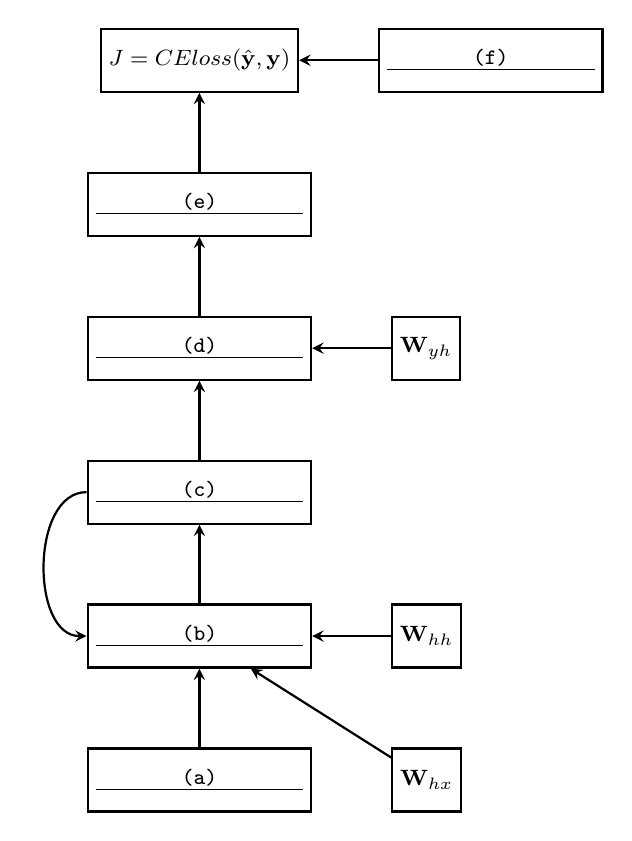
\begin{tikzpicture}[->,
            > = stealth,
            shorten > = 0pt,
            auto,
            thick
        ]\footnotesize

        \tikzstyle{every state}=[
            draw = black,
            thick,
            fill = white,
            minimum size = 0.8cm,
            shape = rectangle
        ]
        \node[state] (B1) {\underline{$~~~~~~~~~~~\textbf{\texttt{(a)}}~~~~~~~~~~~$}}; 
        \node[state] (B2) [above = \distV of B1] {\underline{$~~~~~~~~~~~\textbf{\texttt{(b)}}~~~~~~~~~~~$}};
        \node[state] (B3) [right = \distV of B2] { $\Wv_{hh}$};
        \node[state] (B4) [below = \distHTwo of B3] {$\Wv_{hx}$};
        \node[state] (B5) [above = \distV of B2] {\underline{$~~~~~~~~~~~\textbf{\texttt{(c)}}~~~~~~~~~~~$}};
        \node[state] (B6) [above = \distV of B5] {\underline{$~~~~~~~~~~~\textbf{\texttt{(d)}}~~~~~~~~~~~$}};
        \node[state] (B7) [right = \distV of B6] {$\Wv_{yh}$};
        \node[state] (B8) [above = \distV of B6] {\underline{$~~~~~~~~~~~\textbf{\texttt{(e)}}~~~~~~~~~~~$}};
        \node[state] (B9) [above = \distV of B8] {$J = CEloss(\hat{\yv},\yv)$};
        \node[state] (B0) [right = \distV of B9] {\underline{$~~~~~~~~~~~\textbf{\texttt{(f)}}~~~~~~~~~~~$}};
        \path
        (B1) edge node [swap] {$ $} (B2)
        (B2) edge node [swap] {$ $} (B5)
        (B5) edge[bend right=90] node [swap] {$ $} (B2)
        (B3) edge node [swap] {$ $} (B2)
        (B4) edge node [swap] {$ $} (B2)
        (B5) edge node [swap] {$ $} (B6)
        (B7) edge node [swap] {$ $} (B6)
        (B6) edge node [swap] {$ $} (B8)
        (B8) edge node [swap] {$ $} (B9)
        (B0) edge node [swap] {$ $} (B9);
    \end{tikzpicture}
    \end{center}
    
    \begin{your_solution}[title=(a),height=2cm,width=4.8cm]
    % YOUR ANSWER
    Input $\xv_1$
    \end{your_solution}
     \begin{your_solution}[title=(b),height=2cm,width=4.8cm]
    % YOUR ANSWER
    $\hv_0 = \vec{0}$
    \end{your_solution}
     \begin{your_solution}[title=(c),height=2cm,width=4.8cm]
    % YOUR ANSWER
    $\zv_1 = \Wv_{hx}\xv_1$
    \end{your_solution}\\
     \begin{your_solution}[title=(d),height=2cm,width=4.8cm]
    % YOUR ANSWER
    $\hv_1 = \psi(\zv_1)$
    \end{your_solution}
     \begin{your_solution}[title=(e),height=2cm,width=4.8cm]
    % YOUR ANSWER
    $\ov_1 = \Wv_{yh}\hv_1$
    \end{your_solution}
     \begin{your_solution}[title=(f),height=2cm,width=4.8cm]
    % YOUR ANSWER
    $-\sum_{i=1}^2 y_{3,i}\log(\hat{y}_{3,i})$
    \end{your_solution}
    
    
    % \subpart Now you will derive the steps of the backpropagation algorithm that lead to the computation of $\frac{dJ}{dW_{hh}}$. For all parts of this question, please write your answer in terms of $W_{hh}$, $W_{yh}$, $y$, $\hat{y}$, $h$, and any additional terms specified in the question (note: this does not mean that every term listed shows up in every answer, but rather that you should simplify terms into these as much as possible when you can).

    % \begin{subsubparts}
    %     \subsubpart[2] Let $J_t = -\sum_{i=1}^2 y_{t,i} \log(\hat{y}_{t,i})$. What is $\frac{\partial J_t}{\partial o_t}$? Write your solution in the first box, and show your work in the second.
    
    % %\emph{(Hint: First derive the partial derivatives with respective to everything after $h_t$, which should be similar to HW5. After that, try to break up the objective into a term for each timestep.)}
    
    % \begin{your_solution}[title=$\frac{\partial J_t}{\partial \ov_t}$,height=2.5cm,width=8.5cm]
    % % YOUR ANSWER
    % \end{your_solution}
    
    % \begin{your_solution}[title=Work,height=6cm,width=14cm]
    % % YOUR ANSWER
    % \end{your_solution}
    
    % \subsubpart[2] Suppose you have a variable $\gv_{\ov_t}$ that stores the value of $\frac{\partial J_t}{\partial \ov_t}$. What is $\frac{\partial J_t}{\partial \hv_i}$ for an arbitrary $i \in [1,3]$? Write your solution in terms of the $\gv_{\ov_t}$ and the aforementioned variables in the first box, and show your work in the second.
    
    % %\emph{(Hint: First derive the partial derivatives with respective to everything after $h_t$, which should be similar to HW5. After that, try to break up the objective into a term for each timestep.)}
    
    % \begin{your_solution}[title=$\frac{\partial J_t}{\partial \hv_i}$,height=2.5cm,width=8.5cm]
    % % YOUR ANSWER
    % \end{your_solution}
    
    % \begin{your_solution}[title=Work,height=6cm,width=14cm]
    % % YOUR ANSWER
    % \end{your_solution}
    
    % \subsubpart[2] Suppose you have a variable $\gv_{\hv_i}$ that stores the value of $\frac{\partial J_t}{\partial \hv_i}$. What is $\frac{\partial J_t}{\partial \Wv_{hh}}$? Write your solution in terms of the $\gv_{\hv_i}$ and the aforementioned variables in the first box, and show your work in the second.
    
    
    % \begin{your_solution}[title=$\frac{\partial J_t}{\partial W_{hh}}$,height=2.5cm,width=10.5cm]
    % % YOUR ANSWER
    % \end{your_solution}
    
    % \begin{your_solution}[title=Work,height=8.5cm,width=14cm]
    % % YOUR ANSWER
    % \end{your_solution}
    
    % \subsubpart[1] Suppose you have a variable $\gv_{W_{hh},t}$ that stores the value of $\frac{\partial J_t}{\partial W_{hh}}$. What is $\frac{\partial J}{\partial \Wv_{hh}}$? Write your solution in terms of the $\gv_{W_{hh},t}$ and the aforementioned variables in the first box, and show your work in the second.
    \subpart[1] 

    For this question, please write your answer in terms of $W_{hh}$, $W_{yh}$, $y$, $\hat{y}$, $h$, and any additional terms specified explicitly (note: this does not mean that every term listed shows up in the answer, but rather that you should simplify terms into these as much as possible when you can).
    
    Suppose you have a variable $\gv_{W_{hh},t}$ that stores the value of $\frac{\partial J_t}{\partial W_{hh}}$. What is $\frac{\partial J}{\partial \Wv_{hh}}$? Write your solution in terms of the $\gv_{W_{hh},t}$ and the aforementioned variables in the first box, and show your work in the second.
    
    \begin{your_solution}[title=$\frac{\partial J}{\partial W_{hh}}$,height=2.5cm,width=10.5cm]
    % YOUR ANSWER

    $\frac{\partial J}{\partial W_{hh}} = \sum_{t=1}^3 \frac{\partial J_t}{\partial W_{hh}} = \gv_{W_{hh},1} + \gv_{W_{hh},2} + \gv_{W_{hh},3}$
    \end{your_solution}
    
    \begin{your_solution}[title=Work,height=4.5cm,width=10.5cm]
    % YOUR ANSWER
    \end{your_solution}
    
    % \end{subsubparts}
    
\end{subparts}

\end{parts}
\newpage

\newcommand \vcdim {\text{VC}(\mathcal{H})}
\sectionquestion{Learning Theory}
\begin{parts}
    \part Neural the Narwhal is given a classification task to solve, which he decides to use a decision tree learner with 2 binary features $X_1$ and $X_2$. On the other hand, you think that Neural should not have used a decision tree. Instead, you think it would be best to use logistic regression with 16 real-valued features in addition to a bias term. You want to use PAC learning to check whether you are correct. You first train your logistic regression model on $N$ examples to obtain a training error $\hat R$. 
    
    \begin{subparts}
    \subpart[1] Which of the following case of PAC learning should you use for your logistic regression model?
    \begin{checkboxes}
        % YOUR ANSWER 
        \choice Finite and realizable
        \choice Finite and agnostic
        \choice Infinite and realizable
        \CorrectChoice Infinite and agnostic
    \end{checkboxes}
    
    \vspace{5mm}
    
    \subpart[2] What is the upper bound on the true error $R$ in terms of $\hat R$, $\delta$, and $N$?  You may use big-$\mathcal{O}$ notation if necessary. Write only the final answer.  Your work will \textit{not} be graded.\\
    \textbf{Note:} Your answer may not contain any other symbols.
     \\
    \begin{your_solution}[height=4cm]
        % YOUR ANSWER 
        $$R(h) \le \hat{R}(h) + O\Bigg(\sqrt{\frac{1}{N}\Big(17 + \log{\frac{1}{\delta}}\Big)}\Bigg) $$
    \end{your_solution}
    
    \vspace{5mm}
    
    \subpart[3] \sone You want to argue your method has a lower bound on the true error as compared to the Neural's true error bound. Assume that you have obtained enough data points to satisfy the PAC criterion with the same $\epsilon$ and $\delta$ as Neural. Which of the following is true?
    \begin{checkboxes}
        % YOUR ANSWER 
        \choice Neural's model will always classify unseen data more accurately because it only needs 2 binary features and therefore is simpler.
        \choice You must first regularize your model by removing 14 features to make any comparison at all.
        \choice It is sufficient to show that the VC dimension of your classifier is higher than that of Neural's, therefore having a lower bound for the true error.
        \CorrectChoice It is necessary to show that the training error you achieve is lower than the training error Neural achieves.
    \end{checkboxes}
    \end{subparts}

\newpage

    \part In lecture, we saw that we can use our sample complexity bounds to derive bounds on the true error for a particular algorithm. Consider the sample complexity bound for the infinite, agnostic case:
$$N = O\left(\frac{1}{\epsilon^2} \left[\vcdim + \log \frac{1}{\delta} \right] \right).$$

    \begin{subparts}
    \subpart[2] What is the big-$\mathcal{O}$ bound of $\epsilon$ in terms of $N$, $\delta$, and $\vcdim$? \\ 
    \textbf{Note:} $A = \mathcal{O}(B)$ (for some value $B$)  $\Leftrightarrow$ there exists a constant $c \in \mathbb{R}$ such that $A \le cB$.
    
    % Note: Your final answer should look like this: $\epsilon = \mathcal{O}(...)$ where the Big-O is filled in accordingly.
    \begin{your_solution}[height=8cm]
        % YOUR ANSWER 
$$\epsilon = \mathcal{O}\left(\frac{1}{\sqrt{\frac{N}{(\vcdim + \log \frac{1}{\delta})}}}\right)$$
    \end{your_solution}
    
    
    \subpart[2] Now, using the definition of $\epsilon$ (i.e. $|R(h) - \hat{R}(h)| \le \epsilon$) and your answer to part a, prove that with probability at least $(1-\delta)$: $$R(h) \le \hat{R}(h) + O\left(\sqrt{\frac{1}{N} \left[\vcdim + \log\frac{1}{\delta} \right]} \right).$$
    \begin{your_solution}[height=20cm]
        % YOUR ANSWER 
    By the definition of $\epsilon$, we have:

    \begin{equation}
    |R(h) - \hat{R}(h)| \le \epsilon.
    \end{equation}
    
    From the previous question, we derived the big-$\mathcal{O}$ bound of $\epsilon$:
    
    \begin{equation}
    \epsilon = \mathcal{O}\left(\frac{1}{\sqrt{\frac{N}{c(\vcdim + \log \frac{1}{\delta})}}}\right).
    \end{equation}
    
    Since $|R(h) - \hat{R}(h)| \le \epsilon$ and we want to prove that with probability at least $(1-\delta)$,
    
    \begin{equation}
    R(h) \le \hat{R}(h) + O\left(\sqrt{\frac{1}{N} \left[\vcdim + \log\frac{1}{\delta} \right]} \right),
    \end{equation}
    
    we can rewrite the inequality from Equation (1) as follows:
    
    \begin{equation}
    R(h) - \hat{R}(h) \le \epsilon.
    \end{equation}
    
    Now, substitute the bound of $\epsilon$ from Equation (2) into Equation (4):
    
    \begin{equation}
    R(h) - \hat{R}(h) \le \mathcal{O}\left(\frac{1}{\sqrt{\frac{N}{\vcdim + \log \frac{1}{\delta}}}}\right).
    \end{equation}
    
    Next, we can simplify the expression inside the big-$\mathcal{O}$ notation:
    
    \begin{equation}
    R(h) - \hat{R}(h) \le \mathcal{O}\left(\sqrt{\frac{1}{N} \left[\vcdim + \log\frac{1}{\delta} \right]} \right).
    \end{equation}
    
    Finally, rearrange the inequality to get the desired result:
    
    \begin{equation}
    R(h) \le \hat{R}(h) + \mathcal{O}\left(\sqrt{\frac{1}{N} \left[\vcdim + \log\frac{1}{\delta} \right]} \right
    \end{equation}
    \end{your_solution}
    \end{subparts}

\part[3] Consider the hypothesis space of functions that map $M$ binary attributes to a binary label. A function $f$ in this space can be characterized as $f: \{0,1\}^M \to \{0,1\}$. Neural the Narwhal says that regardless of the value of $M$, a function in this space can always shatter $2^M$ points. Is Neural wrong? If so, provide a counterexample. If Neural is right, briefly explain why in 1-2 \emph{concise} sentences.
    \begin{your_solution}[height=10cm]
        % YOUR ANSWER 
        Neural the Narwhal is right. Given any set of $2^M$ points, we can construct a decision tree with $M$ levels that correctly classifies all of them. Each level of the decision tree corresponds to a different attribute, and the decision at each level splits the set of points based on the value of that attribute. Since there are $2^M$ possible combinations of attribute values, the decision tree can classify all $2^M$ points. Since decision trees correspond to a hypothesis space of functions that map $M$ binary attributes to a binary label, this shows that such a function can shatter $2^M$ points.

    \end{your_solution}
    
\part Consider an instance space $\Xc$ which is the set of real numbers. 

\begin{subparts}
\subpart[3] \sone What is the VC dimension of hypothesis class $H$, where each hypothesis $h$ in $H$ is of the form  ``if $a < x < b$ or $c < x < d$ then $y = 1$; otherwise $y = 0$"?  (i.e., $H$ is an infinite hypothesis class where $a, b, c$, and $d$ are arbitrary real numbers).
    \begin{checkboxes}
        % YOUR ANSWER 
        \choice $2$
        \choice $3$
        \CorrectChoice $4$
        \choice $5$
        \choice $6$
    \end{checkboxes}

\subpart[3] Given the set of points in $\Xc$ below, construct a labeling of some subset of the points to show that any dimension larger than the VC dimension of $H$ by \emph{exactly} 1 is incorrect (e.g. if the VC dimension of $H$ is 3, only fill in the answers for 4 of the points). Fill in the boxes such that for each point in your example, the corresponding label is either $0$ or $1$. For points you are not using in your example, write N/A (do \textit{not} leave the answer box blank).

\usetikzlibrary{arrows}
\begin{center}
\begin{tikzpicture}[scale=2]
\draw[latex-latex] (-3.5,0) -- (3.5,0) ; %edit here for the axis
\foreach \x in  {-3,-2,-1,0,1,2,3} % edit here for the vertical lines
\draw[shift={(\x,0)},color=black] (0pt,3pt) -- (0pt,-3pt);
\foreach \x in {-3,-2,-1,0,1,2,3} % edit here for the numbers
\draw[shift={(\x,0)},color=black] (0pt,0pt) -- (0pt,-3pt) node[below] 
{$\x$};
\draw[o-o] (-3,0.0425);
\draw[o-o] (-2,0.0425);
\draw[o-o] (-1,0.0425);
\draw[o-o] (0,0.0425);
\draw[o-o] (1,0.0425);
\draw[o-o] (2,0.0425);
\draw[o-o] (3,0.0425);
\end{tikzpicture}
\end{center}

    \begin{your_solution}[title=Answer for $-3$,width=3.5cm,height=2cm]
        % Your answer for -3
        % If you do not wish to use this point, write N/A.
        1
    \end{your_solution}
    \begin{your_solution}[title=Answer for $-2$,width=3.5cm,height=2cm]
        % Your answer for -2
        % If you do not wish to use this point, write N/A.
        0
    \end{your_solution}
    \begin{your_solution}[title=Answer for $-1$,width=3.5cm,height=2cm]
        % Your answer for -1
        % If you do not wish to use this point, write N/A.
        1
    \end{your_solution}
    
    % DO NOT DELETE THIS SPACE HERE!
    
    \begin{your_solution}[title=Answer for $0$,width=3.5cm,height=2cm]
        % Your answer for 0
        % If you do not wish to use this point, write N/A.
        0
    \end{your_solution}
    \begin{your_solution}[title=Answer for $1$,width=3.5cm,height=2cm]
        % Your answer for 1
        % If you do not wish to use this point, write N/A.
        1
    \end{your_solution}
    \begin{your_solution}[title=Answer for $2$,width=3.5cm,height=2cm]
        % Your answer for 2
        % If you do not wish to use this point, write N/A.
        N/A
    \end{your_solution}
    \begin{your_solution}[title=Answer for $3$,width=3.5cm,height=2cm]
        % Your answer for 3
        % If you do not wish to use this point, write N/A.
        N/A
    \end{your_solution}

\end{subparts}

\end{parts}
\newpage
\sectionquestion{MLE/MAP}
\begin{parts}
    \part[1] \textbf{True or False:} Suppose you place a Beta prior over the Bernoulli distribution, and attempt to learn the parameter $\theta$ of the Bernoulli distribution from data. Further suppose an adversary chooses ``bad'' but finite hyperparameters for your Beta prior in order to confuse your learning algorithm. As the number of training examples grows to infinity, the MAP estimate of $\theta$ can still converge to the MLE estimate of $\theta$.
    \begin{checkboxes}
        \CorrectChoice True
        \choice False
    \end{checkboxes}
    
    
    \part[2] \sone Let $\Gamma$ be a random variable with the following probability density function (pdf): 
    \begin{align*}
        f(\gamma) &= 
        \begin{cases}
        2\gamma  & \text{if } 0 \leq \gamma \leq 1 \\
        0  & \text{otherwise}
        \end{cases}
    \end{align*}
    Suppose another random variable $Y$, which is conditioning on $\Gamma$, follows an exponential distribution with  $\lambda=3\gamma$. Recall that the exponential distribution with parameter $\lambda$ has the following pdf:
    \begin{align*}
        f_{exp}(y) &= 
        \begin{cases}
        \lambda e^{-\lambda y}  & \text{if } y\geq 0 \\
        0  & \text{otherwise}
        \end{cases}
    \end{align*}
    What is the MAP estimate of $\gamma$ given $Y=\frac{2}{3}$ is observed? \\
    \begin{your_solution}[width=4cm,height=2cm]
        % YOUR ANSWER 
        1
    \end{your_solution}
    
    
    \part[4] Neural the Narwhal found a mystery coin and wants to know the probability of landing on heads by flipping this coin. He models the coin toss as sampling a value from $\text{Bernoulli}(\theta)$ where $\theta$ is the probability of heads. He flips the coin three times and the flips turned out to be heads, tails, and heads. An oracle tells him that $\theta \in \{0, 0.25, 0.5, 0.75, 1\}$, and \textit{no other values of $\theta$ should be considered}.
    
    Find the MLE and MAP estimates of $\theta$. Use the following prior distribution for the MAP estimate:
    \[
    p(\theta)= \begin{cases} 0.9 & \text{if } \theta = 0\\ 0.04 & \text{if } \theta = 0.25\\ 0.03 & \text{if } \theta = 0.5 \\ 0.02 & \text{if } \theta = 0.75\\  0.01 & \text{if } \theta = 1 \end{cases}.
    \]
    Again, remember that $\theta \in \{0, 0.25, 0.5, 0.75, 1\}$, so the MLE and MAP should also be one of them.
    
    \begin{your_solution}[title=MLE of $\theta$,width=4cm,height=2cm]
        % Your answer for MLE
        0.5
    \end{your_solution}
    \begin{your_solution}[title=MAP of $\theta$,width=4cm,height=2cm]
        % Your answer for MAP
        0.5
    \end{your_solution}
    
    
    \newpage
    
    \part In a previous homework assignment, you have derived the closed form solution for linear regression. Now, we are coming back to linear regression, viewing it as a statistical model, and deriving the MLE and MAP estimate of the parameters in the following questions. 
    
    As a reminder, in MLE, we have
    \begin{align*}
        \hat{\theta}_{MLE} &= \argmax_\theta p(D | \theta)
    \end{align*}
    For MAP, we have
    \begin{align*}
        \hat{\theta}_{MAP} &= \argmax_\theta p(\theta| D)
    \end{align*}
    
    Assume we have data $D = \{\mathbf{x}^{(i)}, y^{(i)}\}_{i=1}^{N}$, where $\mathbf{x}^{(i)} = (x_1^{(i)}, \cdots, x_M^{(i)})$. So our data has $N$ instances and each instance has $M$ features. Each $y^{(i)}$ is generated given $\mathbf{x}^{(i)}$ with additive noise $\epsilon^{(i)} \sim \Nc(0, \sigma^2)$: that is, $y^{(i)} = \mathbf{w}^T \mathbf{x}^{(i)} + \epsilon^{(i)}$ where $\mathbf{w}$ is the parameter vector of linear regression.
    \begin{subparts}
    \subpart[2] \sone Given this assumption, what is the distribution of $y^{(i)}$? 
    \begin{checkboxes}
        % YOUR ANSWER 
        \CorrectChoice $y^{(i)} \sim \Nc(\mathbf{w}^T \mathbf{x}^{(i)}, \sigma^2)$
        \choice $y^{(i)} \sim \Nc(0, \sigma^2)$
        \choice $y^{(i)} \sim \text{Uniform}(\mathbf{w}^T \mathbf{x}^{(i)} - \sigma,  \mathbf{w}^T \mathbf{x}^{(i)} + \sigma)$
        \choice None of the above
    \end{checkboxes}
    
    
    \vspace{5mm}
    
    \subpart[2] \sone The next step is to learn the MLE of the parameters of the linear regression model. Which expression below is the correct conditional log likelihood $\ell(\mathbf{w})$ with the given data?
    \begin{checkboxes}
        % YOUR ANSWER 
        \CorrectChoice $\sum_{i=1}^{N} [-\log (\sqrt{2\pi\sigma^2}) - \frac{1}{2\sigma^2} (y^{(i)} - \mathbf{w}^T\mathbf{x}^{(i)})^2]$
        \choice $\sum_{i=1}^{N} [\log (\sqrt{2\pi\sigma^2}) + \frac{1}{2\sigma^2} (y^{(i)} - \mathbf{w}^T\mathbf{x}^{(i)})^2]$
        \choice $\sum_{i=1}^{N} [-\log(\sqrt{2\pi\sigma^2)} - \frac{1}{2\sigma^2} (y^{(i)} - \mathbf{w}^T\mathbf{x}^{(i)})]$
        \choice $-\log (\sqrt{2\pi\sigma^2}) + \sum_{i=1}^{N} [-\frac{1}{2\sigma^2} (y^{(i)} - \mathbf{w}^T\mathbf{x}^{(i)})^2]$
    \end{checkboxes}
    
    
    \vspace{5mm}
    
    \subpart[3] \sall Then, the MLE of the parameters is just  $\argmax_{\mathbf{w}} \ell(\mathbf{w})$. Among the following expressions, select ALL that can yield the correct MLE.
    {\checkboxchar{$\Box$} \checkedchar{$\blacksquare$}
    \begin{checkboxes}
        % YOUR ANSWER 
        \choice $\argmax_{\mathbf{w}} \sum_{i=1}^{N} [-\log (\sqrt{2\pi\sigma^2}) - \frac{1}{2\sigma^2} (y^{(i)} - \mathbf{w}^T\mathbf{x}^{(i)})]$
        \CorrectChoice $\argmax_{\mathbf{w}} \sum_{i=1}^{N} [-\log (\sqrt{2\pi\sigma^2}) - \frac{1}{2\sigma^2} (y^{(i)} - \mathbf{w}^T\mathbf{x}^{(i)})^2]$
        \CorrectChoice $\argmax_{\mathbf{w}} \sum_{i=1}^{N} [- \frac{1}{2\sigma^2} (y^{(i)} - \mathbf{w}^T\mathbf{x}^{(i)})^2]$
        \choice $\argmax_{\mathbf{w}} \sum_{i=1}^{N} [- \frac{1}{2} (y^{(i)} - \mathbf{w}^T\mathbf{x}^{(i)})]$
        \CorrectChoice $\argmax_{\mathbf{w}} \sum_{i=1}^{N} [- \frac{1}{2} (y^{(i)} - \mathbf{w}^T\mathbf{x}^{(i)})^2]$
        \choice None of the above
    \end{checkboxes}
    }
    \end{subparts}

\newpage
    \part Now we are moving on to learn the MAP estimate of the parameters of the linear regression model. Consider the same data $D$ we used for the previous problem.
    
    \begin{subparts}
    \subpart[3] \sall Which expression below is the correct optimization problem the MAP estimate is trying to solving? Recall that $D$ refers to the data, and $\mathbf{w}$ to the regression parameters (weights).
    {\checkboxchar{$\Box$} \checkedchar{$\blacksquare$}
    \begin{checkboxes}
        % YOUR ANSWER 
        \CorrectChoice $\mathbf{w}_{MAP} = \arg\max_{\mathbf{w}} p(D, \mathbf{w})$
        \CorrectChoice $\mathbf{w}_{MAP} = \arg\max_{\mathbf{w}} \frac{p(D| \mathbf{w})p(\mathbf{w})}{p(D)}$
        \choice $\mathbf{w}_{MAP} = \arg\max_{\mathbf{w}} \frac{p(D, \mathbf{w})}{p(\mathbf{w})}$
        \CorrectChoice $\mathbf{w}_{MAP} = \arg\max_{\mathbf{w}} p(D| \mathbf{w})p(\mathbf{w})$
        \CorrectChoice $\mathbf{w}_{MAP} = \arg\max_{\mathbf{w}} p(\mathbf{w}| D)$
        \choice None of the above
    \end{checkboxes}
    }
    

    \subpart[3] \sone Suppose we are using a Gaussian prior distribution with mean $0$ and variance $\frac{1}{\lambda}$ for each element $w_m$  of the parameter vector $\mathbf{w}$, i.e. $w_m \sim \mathcal{N}\left(0, \frac{1}{\lambda}\right)$ $(1 \leq m \leq M )$. Assume that $w_1, \cdots, w_M$ are mutually independent of each other. Which expression below is the correct log joint-probability of the data and parameters $\log p(D, \mathbf{w})$?  Please show your work below.
    \begin{checkboxes}
        % YOUR ANSWER 
        \choice $\sum_{i=1}^N\left(-\log (\sqrt{2\pi\sigma^2}) - \frac{1}{2\sigma^2} (y^{(i)} - \mathbf{w}^T\mathbf{x}^{(i)})^2\right) - \sum_{m=1}^M \log(\sqrt{2\pi\lambda}) - \lambda (w_m)^2$
        \choice $\sum_{i=1}^N\left(-\log (\sqrt{2\pi\sigma^2}) - \frac{1}{2\sigma^2} (y^{(i)} - \mathbf{w}^T\mathbf{x}^{(i)})\right) + \sum_{m=1}^M -\log(\sqrt{2\pi\lambda}) - \lambda (w_m)^2$
        \choice $\sum_{i=1}^N\left(-\log (\sqrt{2\pi\sigma^2}) - \frac{1}{2\sigma^2} (y^{(i)} - \mathbf{w}^T\mathbf{x}^{(i)})\right) -  \sum_{m=1}^M \log(\sqrt{\frac{2\pi}{\lambda}}) - \frac{\lambda}{2}(w_m)^2$
        \CorrectChoice $\sum_{i=1}^N\left(-\log (\sqrt{2\pi\sigma^2}) - \frac{1}{2\sigma^2} (y^{(i)} - \mathbf{w}^T\mathbf{x}^{(i)})^2\right) +  \sum_{m=1}^M -\log(\sqrt{\frac{2\pi}{\lambda}}) - \frac{\lambda}{2}(w_m)^2$
    \end{checkboxes}
    
     \begin{your_solution}[title=Work,height=15cm]
        % YOUR ANSWER
        The log joint probability of the data and parameters is given by:
\begin{align*}
\log p(D, \mathbf{w}) &= \log p(D|\mathbf{w}) + \log p(\mathbf{w})\\
&= \log \left(\prod_{i=1}^N p(y^{(i)}|\mathbf{x}^{(i)}, \mathbf{w})\right) + \log \left(\prod_{m=1}^M p(w_m)\right)\\
&= \sum_{i=1}^N\log p(y^{(i)}|\mathbf{x}^{(i)}, \mathbf{w}) + \sum_{m=1}^M\log p(w_m)\\
&= \sum_{i=1}^N\log \left(\frac{1}{\sqrt{2\pi\sigma^2}}\exp\left(-\frac{(y^{(i)} - \mathbf{w}^T\mathbf{x}^{(i)})^2}{2\sigma^2}\right)\right) + \sum_{m=1}^M\log \left(\frac{1}{\sqrt{2\pi/\lambda}}\exp\left(-\frac{\lambda (w_m)^2}{2}\right)\right)\\
&= \sum_{i=1}^N\left(-\log (\sqrt{2\pi\sigma^2}) - \frac{1}{2\sigma^2} (y^{(i)} - \mathbf{w}^T\mathbf{x}^{(i)})^2\right) + \sum_{m=1}^M\left(-\log(\sqrt{2\pi/\lambda}) - \frac{\lambda}{2}(w_m)^2\right)\\
&= \sum_{i=1}^N\left(-\log (\sqrt{2\pi\sigma^2}) - \frac{1}{2\sigma^2} (y^{(i)} - \mathbf{w}^T\mathbf{x}^{(i)})^2\right) + \sum_{m=1}^M -\log(\sqrt{\frac{2\pi}{\lambda}}) - \frac{\lambda}{2}(w_m)^2
\end{align*}

Therefore, the correct expression for the log joint-probability of the data and parameters is:
        $\sum_{i=1}^N\left(-\log (\sqrt{2\pi\sigma^2}) - \frac{1}{2\sigma^2} (y^{(i)} - \mathbf{w}^T\mathbf{x}^{(i)})^2\right) + \sum_{m=1}^M -\log(\sqrt{\frac{2\pi}{\lambda}}) - \frac{\lambda}{2}(w_m)^2$
    \end{your_solution}
        
    
    \newpage
    \subpart[2] \sone For the same linear regression model with a Gaussian prior on the parameters as in the previous question, maximizing the log posterior probability  $\ell_{\textit{MAP}}(\mathbf{w})$ gives you the MAP estimate of the parameters.
    Which of the following is an equivalent definition of  $\max_{\mathbf{w}} \ell_{\textit{MAP}}(\mathbf{w})$?
    \begin{checkboxes}
        % YOUR ANSWER 
        \choice $\max_{\mathbf{w}} \sum_{i=1}^N\frac{1}{2\sigma^2} (y^{(i)} - \mathbf{w}^T\mathbf{x}^{(i)})^2 + \frac{\lambda}{2}\|\mathbf{w}\|_2^2$
        \CorrectChoice $\min_{\mathbf{w}} \sum_{i=1}^N\frac{1}{2\sigma^2} (y^{(i)} - \mathbf{w}^T\mathbf{x}^{(i)})^2 + \frac{\lambda}{2}\|\mathbf{w}\|_2^2$
        \choice $\max_{\mathbf{w}} \sum_{i=1}^N\frac{1}{2\sigma^2} (y^{(i)} - \mathbf{w}^T\mathbf{x}^{(i)})^2 + \lambda\|\mathbf{w}\|_2^2$
        \choice $\min_{\mathbf{w}} - \sum_{i=1}^N\frac{1}{2\sigma^2} (y^{(i)} - \mathbf{w}^T\mathbf{x}^{(i)})^2 - \frac{\lambda}{2}\|\mathbf{w}\|_2^2$
    \end{checkboxes}
    
    
    \vspace{2mm}

    \subpart[2] \sone You found a MAP estimator that has a much higher test error than train error using some Gaussian prior. Which of the following could be a possible approach to fixing this?
    \begin{checkboxes}
        % YOUR ANSWER 
        \choice Increase the variance of the prior used
        \CorrectChoice Decrease the variance of the prior used
    \end{checkboxes}
    
    \end{subparts}

    
    \vspace{2mm}
    
    \part[4] \sone Suppose now the additive noise $\epsilon$ is different per datapoint. That is, each $y^{(i)}$ is generated given $\mathbf{x}^{(i)}$ with additive noise $\epsilon^{(i)} \sim \Nc(0, \sigma_i^2)$, i.e. $y^{(i)} = \mathbf{w}^T \mathbf{x}^{(i)} + \epsilon^{(i)}$. Unlike the standard regression model we have worked with until now, there is now an example specific variance $\sigma_i^2$. Maximizing the log-likelihood of this new model is equivalent to minimizing the \textit{weighted} mean squared error with which of the following as the weights? Please show your work below.
    \begin{checkboxes}
        % YOUR ANSWER 
        \choice $1/y^{(i)}$
        \CorrectChoice $1/\sigma_i^2$
        \choice $1/\|\xv^{(i)}\|_2^2$
    \end{checkboxes}
    \vspace*{-2mm}
    \begin{your_solution}[title=Work,height=9.8cm]
        % YOUR ANSWER
        The log-likelihood function of the new model is given by:
\begin{align*}
\log p(D|\mathbf{w}) &= \sum_{i=1}^N\log p(y^{(i)}|\mathbf{x}^{(i)}, \mathbf{w}) \\
&= \sum_{i=1}^N\log \left(\frac{1}{\sqrt{2\pi\sigma_i^2}}\exp\left(-\frac{(y^{(i)} - \mathbf{w}^T\mathbf{x}^{(i)})^2}{2\sigma_i^2}\right)\right) \\
&= \sum_{i=1}^N\left(-\log (\sqrt{2\pi\sigma_i^2}) - \frac{1}{2\sigma_i^2} (y^{(i)} - \mathbf{w}^T\mathbf{x}^{(i)})^2\right) \\
&= -\frac{1}{2} \sum_{i=1}^N \log (2\pi\sigma_i^2) - \frac{1}{2} \sum_{i=1}^N \frac{(y^{(i)} - \mathbf{w}^T\mathbf{x}^{(i)})^2}{\sigma_i^2}
\end{align*}
Therefore, maximizing the log-likelihood of this new model is equivalent to minimizing the weighted mean squared error with weights $1/\sigma_i^2$.
    \end{your_solution}
    
    \newpage
    
    \part[4] \sone MAP estimation with what prior is equivalent to $\ell_1$ regularization?  Please show your work below.

    Note:
    \begin{itemize}
    \item The pdf of a uniform distribution over $[a,b]$ is $f(x) = \frac{1}{b-a}$ if $x \in [a,b]$ and $0$ otherwise.
    \item The pdf of an exponential distribution with rate parameter $a$ is $f(x) = a \exp(-a x)$ for $x > 0$.
    \item The pdf of a Laplace distribution with location parameter $a$ and scale parameter $b$ is \\$f(x) = \frac{1}{2b} \exp \left( \frac{- |x - a| }{b} \right)$ for all $x \in \mathbb{R}$.
    \end{itemize}
    
    \begin{checkboxes}
        % YOUR ANSWER 
        \choice Uniform distribution over $[-1, 1]$
        \choice Uniform distribution over $\left[- \mathbf{w}^T\mathbf{x}^{(i)}, \mathbf{w}^T\mathbf{x}^{(i)} \right]$
        \choice Exponential distribution with rate parameter $a = \frac{1}{2}$
        \choice Exponential distribution with rate parameter $a = \mathbf{w}^T \mathbf{x}^{(i)}$
        \CorrectChoice Laplace distribution with location parameter $a = 0$
        \choice Laplace distribution with location parameter $a = \mathbf{w}^T \mathbf{x}^{(i)}$
    \end{checkboxes}
    
    \begin{your_solution}[title=Work,height=13cm]
        % YOUR ANSWER
        MAP estimation with a Laplace prior distribution with location parameter $a=0$ is equivalent to $\ell_1$ regularization.

The MAP estimation with a Laplace prior is given by:
\begin{align*}
\hat{\mathbf{w}} &= \arg\max_{\mathbf{w}} p(\mathbf{w}|D)\\
&= \arg\max_{\mathbf{w}} p(D|\mathbf{w}) p(\mathbf{w})\\
&= \arg\max_{\mathbf{w}} \left(\prod_{i=1}^N p(y^{(i)}|\mathbf{x}^{(i)}, \mathbf{w})\right) \left(\prod_{m=1}^M p(w_m)\right)\\
&= \arg\max_{\mathbf{w}} \left(\prod_{i=1}^N \frac{1}{\sqrt{2\pi}\sigma} \exp\left(-\frac{(y^{(i)} - \mathbf{w}^T\mathbf{x}^{(i)})^2}{2\sigma^2}\right)\right) \left(\prod_{m=1}^M \frac{1}{2b} \exp\left(-\frac{|w_m|}{b}\right)\right)\\
&= \arg\min_{\mathbf{w}} \frac{1}{2\sigma^2} \sum_{i=1}^N (y^{(i)} - \mathbf{w}^T\mathbf{x}^{(i)})^2 + \frac{1}{b} \sum_{m=1}^M |w_m|\\
&= \arg\min_{\mathbf{w}} \frac{1}{2\sigma^2} | \yv - X \mathbf{w} |_2^2 + \lambda | \mathbf{w} |_1,
\end{align*}
where $b=\lambda/\sigma^2$ is the scale parameter of the Laplace distribution, and $\lambda$ is the regularization parameter.
the Laplace prior with location parameter $a=0$ is equivalent to $\ell_1$ regularization
    \end{your_solution}
\end{parts}\newpage
\sectionquestion{Naïve Bayes}
\begin{parts}
    % \part[3] Suppose that 0.3\% of all people have cancer. If someone is tested for cancer, the outcome of the test can either be positive (cancer) or negative (no cancer). The test is not perfect---among people who have cancer, the test comes back positive 97\% of the time. Among people who don’t have cancer, the test comes back positive 4\% of the time. For this question, you should assume that the test results are independent of each other, given the true state (cancer or no cancer). What is the probability of a test subject having cancer, given that the subject’s test result is positive? Round the answer to the fourth decimal place, e.g. 0.1234. \\
    % \begin{your_solution}[width=4cm,height=2cm, title = $P(C{,} +)$]
    %     % YOUR ANSWER 
    % \end{your_solution}
    % \begin{your_solution}[width=4cm,height=2cm, title = $P(+)$]
    %     % YOUR ANSWER 
    % \end{your_solution}
    % \begin{your_solution}[width=4cm,height=2cm, title = $P(C\mid +)$]
    %     % YOUR ANSWER 
    % \end{your_solution}
    
        
    
        
\part The following dataset describes several features of a narwhal and then whether or not it has an Instagram account. 
\begin{center}
\begin{tabular}{|c|c||c|}
\hline
\textbf{Color} & \textbf{Size} & \textbf{Has Instagram?} \\ \hline\hline
Rainbow & Small & N \\ \hline
Cyan & Small &  N \\ \hline
Cyan & Small &  Y \\ \hline
Cyan & Medium &  Y     \\ \hline
Rainbow & Medium & N     \\ \hline
Fuchsia & Medium & Y     \\ \hline
Fuchsia & Large & Y     \\ \hline
Cyan & Large & Y     \\ \hline
\end{tabular}
\end{center}
Neural the Narwhal is cyan and medium-sized. We would like to determine whether he has an Instagram account, using the Naïve Bayes assumption to estimate the following probabilities.

\begin{subparts}
    \subpart[2] What is the probability that a narwhal is cyan, medium-sized, and has an Instagram account? Round the answer to the fourth decimal place, e.g. 0.1234.  \\
    \begin{your_solution}[width=4cm,height=2cm]
        % YOUR ANSWER 
        0.1172
    \end{your_solution}
    
    
    \subpart[2] What is the probability that a narwhal is cyan, medium-sized, and does \textit{not} have an Instagram account? Round the answer to the fourth decimal place, e.g. 0.1234.  \\
    \begin{your_solution}[width=4cm,height=2cm]
        % YOUR ANSWER 
        0.0703
    \end{your_solution}
    
    
    \subpart[1] \sone Does Neural the Narwhal have an Instagram account? 
    \begin{checkboxes}
        % YOUR ANSWER 
        \CorrectChoice Yes
        \choice No
    \end{checkboxes}
    

    \subpart[1] What is the generative story for this data? Name the distributions for the features and labels. Let Y represent whether or not a narwhal has an Instagram account and $X_1$ and $X_2$ represent Color and Size, respectively.

    \begin{your_solution}[width=5cm,height=5cm, title=Y]
        % % YOUR ANSWER 
        $Y \sim Bernoulli(\theta)\\$
        $\theta$ is the probability of a narwhal having an Instagram account
    \end{your_solution}
    \begin{your_solution}[width=4cm,height=5cm, title = $X_1|Y$]
        % % YOUR ANSWER 
        $P(X_1|Y)\\ \sim Categorical(\phi_{X_1|Y})\\$
        $\phi_{X_1|Y}$ is the probability distribution of colors given the Instagram account status (Y)
    \end{your_solution}
    \begin{your_solution}[width=4cm,height=5cm, title = $X_2|Y$]
        % % YOUR ANSWER 
        $P(X_2|Y)\\ \sim Categorical(\phi_{X_2|Y})\\$
        $\phi_{X_2|Y}$ is the probability distribution of sizes given the Instagram account status (Y)
    \end{your_solution}


    \subpart[1] How many parameters do we need to estimate? \\
    \begin{your_solution}[width=4cm,height=2cm]
    % YOUR ANSWER 
    9
    \end{your_solution}


    \subpart[1] Suppose we use Maximum Likelihood Estimation to train our model. What is our estimate of $\theta_{X_1 = \text{ Rainbow}, Y = N}$? \\
    \begin{your_solution}[width=4cm,height=2cm]
    % YOUR ANSWER 
    $\frac{1}{2}$
    \end{your_solution}


    \subpart[1] What is our MLE estimate of $\theta_{X_1 = \text{ Fuchsia}, Y = N}$? \\
    \begin{your_solution}[width=4cm,height=2cm]
    % YOUR ANSWER 
    $\frac{0}{2} = 0$

    \end{your_solution}


    \subpart[1] Give a test data point for which a Naïve Bayes model trained via MLE will never predict the correct label\\
    \begin{your_solution}[width=8cm,height=2cm]
    % YOUR ANSWER 
    Color = Rainbow, Size = Large, Has Instagram? = Y

    \end{your_solution}


    
\end{subparts}



    \part[3] \sall Gaussian Naïve Bayes in general can learn non-linear decision boundaries. Consider the simple case where we have just one real-valued feature $X_1\in\mathbb{R}$ from which we wish to infer the value of label $Y\in\{0,1\}$. The corresponding generative story would be:
    \begin{align*}
    Y &\sim \text{Bernoulli}(\phi) \\
    X_1|Y &\sim \text{Gaussian}\left(\mu_y, \sigma^2_y\right)
    \end{align*}
    where the parameters are the Bernoulli parameter $\phi$ and the class-conditional Gaussian parameters $\mu_0, \sigma^2_0$ and $\mu_1, \sigma^2_1$ corresponding to $Y=0$ and $Y=1$, respectively.
    
    A linear decision boundary in one dimension can be described by a rule of the form: 
    \begin{center}
    if $X_1>c$ then $Y=1$, else $Y=0$
    \end{center}
    where $c$ is a real-valued threshold and $k \in \{0, 1\}$. 
    % Note that $X_1 > c$ here denotes a generic linear inequality. That is, we use $X_1 > c$ to mean any of $X_1 > c$, $X_1 \ge c$, $X_1 < c$, and $X_1 \le c$.
    
    Is it possible in this simple one-dimensional case to construct a Gaussian Naïve Bayes classifier with a decision boundary that cannot be expressed by a rule in the above form? (Hint: Think about what a Gaussian distribution looks like for one random variable)

    {\checkboxchar{$\Box$} \checkedchar{$\blacksquare$}
    \begin{checkboxes}
        % YOUR ANSWER 
        \choice Yes, this can occur if the Gaussians are of equal means and unequal variances.
        \CorrectChoice Yes, this can occur if the Gaussians are of unequal means and equal variances. 
        \CorrectChoice Yes, this can occur if the Gaussians are of unequal means and unequal variances.
        \choice None of the above
    \end{checkboxes}}
    
    

    % \part Now we will expand this to 2D and derive the decision boundary of a 2D Gaussian Naïve Bayes.
    % \begin{subparts}
    %     \subpart[3] Show that the decision boundary of a 2D Gaussian Naïve Bayes classifier is quadratic. That is, show that $p(y=1 \mid x_1, x_2) = p(y=0 \mid x_1, x_2)$ can be written as a polynomial function of $x_1$ and $x_2$ where the degree of each variable is at most 2. You may fold \textit{unimportant} constants into terms such as $C, C', C'', C'''$ so long as \textit{you are clearly showing each step}.\\
    %     \begin{your_solution}[height=9cm]
    %         % YOUR ANSWER 
    %     \end{your_solution}
        
        
        \part[2] \sall Select all possible decision boundaries that can be produced by a Gaussian Naïve Bayes classifier. The shaded region is assigned class 1 and the unshaded regions is assigned class 0. \emph{(Hint: Recall the conclusion of the proof given in recitation.)} 
    \begin{figure}[H]
        \centering
        \includegraphics[scale=0.43]{figs/GNB_decision_boundary.png}
    \end{figure}
    {\checkboxchar{$\Box$} \checkedchar{$\blacksquare$}
    \begin{checkboxes}
        % YOUR ANSWER 
        \CorrectChoice (a)
        \CorrectChoice (b)
        \choice (c)
        \CorrectChoice (d)
        \choice None of the above
    \end{checkboxes}
    }
    
    
    % \end{subparts}

    
    \part Suppose we want to extend the Naïve Bayes model to time series data. Formally, a training data point consists of a binary label Y and D sequentially ordered observations of a binary outcome where $X_1$ occurs before $X_2$, which occurs before $X_3$ and so on all the way down to the final observation $X_D$; each feature $X_d$ is binary. \\

    You decide to modify the Naïve Bayes assumption such that a feature $X_d$ is conditionally independent of all other features given the label Y and the previous feature $X_{d-1}$; the first feature $X_1$ is conditionally independent of all other features given just the label Y. The corresponding Generative story would be: 
    \begin{align*}
    Y &\sim \text{Bernoulli}(\phi) \\
    X_1|Y &\sim \text{Bernoulli}(\theta_{1})\\
    X_d | X_{d-1},Y & \sim \text{Bernoulli}(\theta_{d,x,y})
    \end{align*}
    where the parameters are the Bernoulli parameter $\phi$ and, the class-conditional Bernoulli parameter $\theta_1$ , and the class-conditional Bernoulli parameters $\theta_{d,x,y}$ for $X_d | X_{d-1} = x, Y = y$. 

    \begin{subparts}
        \subpart[2] Write down the expression for the joint distribution $P(X,Y)$ under your new Naïve Bayes model. You must use the modified Naïve Bayes assumption described above \\
        \begin{your_solution}[height=8cm]
        % YOUR ANSWER 

Under the new Naïve Bayes model, the joint distribution $P(X, Y)$ can be expressed as:

\begin{align*}
P(X, Y) &= P(Y)P(X_1|Y)\prod_{d=2}^{D}P(X_d|X_{d-1}, Y) \\
&= \text{Bernoulli}(Y;\phi)\text{Bernoulli}(X_1;\theta_{1,Y})\prod_{d=2}^{D}\text{Bernoulli}(X_d;\theta_{d,X_{d-1},Y})
\end{align*}

where $D$ is the total number of features, and the parameters $\phi$, $\theta_{1,Y}$, and $\theta_{d,X_{d-1},Y}$ are the Bernoulli parameters for the respective distributions.

        \end{your_solution}
        

        \subpart[1] How many parameters do you need to learn in order to make predictions using this new Naïve Bayes model? Write your answer in terms of D.\\
        \begin{your_solution}[width = 4cm,height=2cm]
        % YOUR ANSWER 
        4D - 2
    
        \end{your_solution}
        

        \subpart[2] Suppose we train this model via MLE. In at most 2 sentences, 
        describe how we would estimate $\phi$\\
        \begin{your_solution}[height=3cm]
        % YOUR ANSWER 
        Count the number of instances with Y=1 and divide it by the total number of instances in the dataset. This provides the proportion of instances with Y=1, which serves as our MLE estimate for $\phi$.
    
        \end{your_solution}


        \subpart[2] In at most 2 sentences, describe how we would estimate $\theta_{d,x,y}$ for $2 \leq d \leq D$ using MLE.\\

        \begin{your_solution}[height=3cm]
        % YOUR ANSWER 
        Count the number of instances with $X_d = 1$, $X_{d-1} = x$, and $Y = y$, and then divide this count by the total number of instances with $X_{d-1} = x$ and $Y = y$. This provides the conditional probability of $X_d = 1$ given $X_{d-1} = x$ and $Y = y$.
    
        \end{your_solution}


        

        
    \end{subparts}
    

 
    
    
    % \part[2] \sall Neural the Narwhal used a 2D Gaussian Naïve Bayes model for a binary classification task, and obtained the following contour plot for the density $f(x_1, x_2 \mid y=+)$. You instantly notice that he made a mistake. Why is his result theoretically impossible to be obtained from a Gaussian Naïve Bayes model?
    % \begin{center}
    %     \includegraphics[width=4cm]{figs/contour.pdf}
    % \end{center}
    % {\checkboxchar{$\Box$} \checkedchar{$\blacksquare$}
    % \begin{checkboxes}
    %     % YOUR ANSWER 
    %     \choice The mean of the distribution should be the mean of all points, not just positive points ($+$)
    %     \choice A Bernoulli Naïve Bayes model should be used instead for discrete labels ($+$ and $-$)
    %     \choice The covariance matrix of the distribution is not a diagonal matrix
    %     \choice None of the above
    % \end{checkboxes}
    % }
    

    
\end{parts}\end{questions}

\newpage
\newpage
\section{Collaboration Questions}
After you have completed all other components of this assignment, report your answers to these questions regarding the collaboration policy. Details of the policy can be found \href{http://www.cs.cmu.edu/~mgormley/courses/10601/syllabus.html}{here}.
\begin{enumerate}
    \item Did you receive any help whatsoever from anyone in solving this assignment? If so, include full details.
    \item Did you give any help whatsoever to anyone in solving this assignment? If so, include full details.
    \item Did you find or come across code that implements any part of this assignment? If so, include full details.
\end{enumerate}

\begin{your_solution}[height=6cm]
% YOUR ANSWER 
no, no, no
\end{your_solution}

\end{document}